\section{Versuchsbeschreibung}

Ziel dieses Versuches ist es, den elektro-optischen Pockelseffekt und den magneto-optischen Faradayeffekt zu untersuchen.
\subsection{Pockelszelle}

\begin{figure}[H]
 \centering
 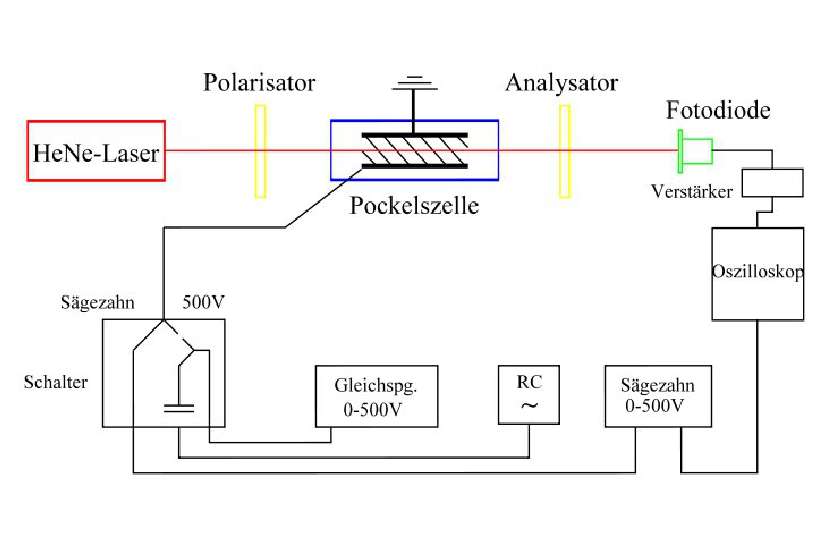
\includegraphics[width=0.9\linewidth]{Bilder/blockbild-pockels.png}
 \caption{Blockbild Pockelseffekt}
\end{figure}

Die Stärke des Pockelseffekts hängt linear mit dem externen E-Feld zusammen und somit ebenfalls von der angelegten Spannung. Wir suchen die Spannungs\-differenz, bei der eine Drehung der Polarisationsebene um $180^{\circ}$ stattfindet ($U_{\lambda/2}$). Das Licht eines Ne-He-Lasers wird durch einen linearen Polarisator geleitet. Wird jetzt die Spannung genau so eingestellt, das sie eine Drehung der Polarisationsebene um $90^{\circ}$ verursacht, erhalten wir durch den Analysator, der ebenfalls um $90^{\circ}$ gedreht ist, ein maximales Signal. Dazu verwenden wir zwei verschiedene Ansätze:
\subsubsection{Sinusspannung}
Auf eine Gleichspannung wird ein kleines Sinussignal aufmodeliert. Stellen wir die den konstanten Untergrund der Spannung genau auf $U_{\lambda/2}/2$ bzw. $-U_{\lambda/2}/2$ ein, so erhalten im Vergleich zur modulierten Sinusspannung eine Frequenzverdopplung, da bei jedem Nulldurchgang der Modulation das Maximum der Intensität erreicht wird.
\subsubsection{Sägezahnspannung}
Es wird eine Sägezahnspannung verwendet, die sowohl eine Drehung um $90^{\circ}$ als auch eine Drehung um $270^{\circ}$ abdeckt. Das Signal der Photodioden zeigt nun einen sinusförmigen Verlauf, mit Extrema bei $90^{\circ}$ und $270^{\circ}$. Durch Abgleich mit der parallel aufgenommenen Sägezahnspannung können wir die gesuchte Spannungsdifferenz ermitteln.
 
\subsection{Faradayeffekt}

\begin{figure}[H]
 \centering
 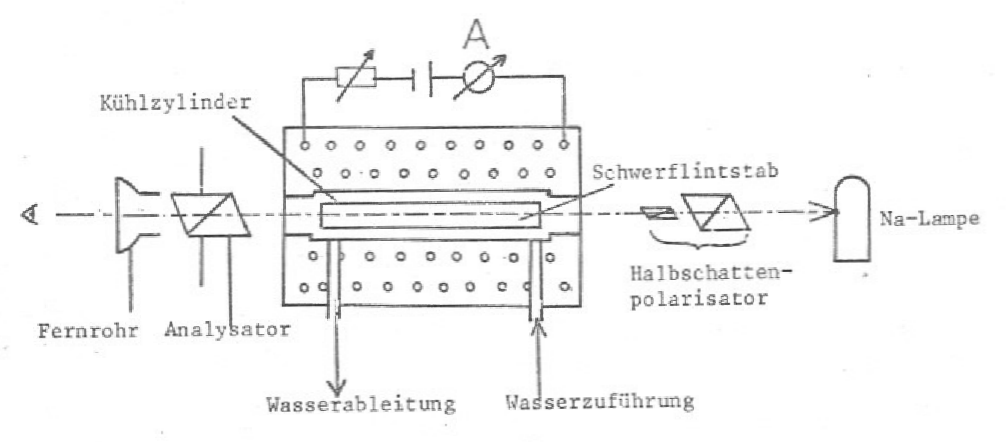
\includegraphics[width=0.9\linewidth]{Bilder/blockbild-faraday.png}
\caption{Blockbild Faradayeffekt}
\end{figure}

Das Licht einer Halogenlampe wird durch einen Schwerflintstab geleitet, der sich im Zentrum einer Spule befindet. Die Stärke des Magnetfeldes kann über die Stromstärke im Bereich von $\pm 4.5A$ eingestellt werden. Wir vermessen dann mit einem Halbschattenpolarimeter die resultierende Drehung der Polarisationsebene in Abhängigkeit von der Stromstärke.
